\documentclass{beamer}

\usepackage{subfigure}
\usepackage{graphicx}
\usepackage{sidecap}
\usepackage{caption}
%\usepackage{subcaption}
\captionsetup{compatibility=false}
\usepackage{appendixnumberbeamer}
\usepackage{amsmath}
% --
\usepackage{multirow}
\usepackage{xcolor}
\usepackage{setspace}
\usepackage{hyperref}
\usepackage{anyfontsize}

\beamertemplatenavigationsymbolsempty
\setbeamertemplate{footline}

\newenvironment{itemise} {\begin{itemize} \setlength{\itemsep}{0.2cm}} {\end{itemize}}
\usepackage[labelformat=empty]{caption}
\setbeamertemplate{sections/subsections in toc}[square]

%% COLORS
\definecolor{Gray}{gray}{0.9}
\definecolor{dblue}{rgb}{0.132,0.1,0.27}
\definecolor{mint}{cmyk}{1.0, 0.2, 0.6, 0.05}
\definecolor{ant}{cmyk}{0.5, 0.1, 0.0, 0.45}
\definecolor{lgray}{cmyk}{0.12, 0.0, 0.0, 0.17}
\definecolor{lred}{cmyk}{0.0, 0.9, 0.7, 0.0}


\usepackage{etoolbox}% http://ctan.org/pkg/etoolbox 
\usepackage{booktabs}

\newenvironment{literatur}{%
  \parskip2pt \parindent0pt \raggedright
  \def\lititem{\hangindent=0.5cm \hangafter1}}{%
  \par\ignorespaces}

\newcommand{\tb}[1]{{\color{blue}{\textbf{#1}}}}
\newcommand{\tm}[1]{{\color{mint}{\textbf{#1}}}}
\newcommand{\tr}[1]{{\color{red}{\textbf{#1}}}}
% Ilya: packages

\usepackage{tikz}
\usepackage{lmodern}
\usepackage{enumitem}

% Ilya: my commands

\newenvironment{mytemize}
{\vfill\itemize[nolistsep,itemsep=\fill,label=\color{blue}{$\triangleright$}]}
  {\enditemize}


\newenvironment{mynumerate}
{\vfill\enumerate[nolistsep,itemsep=\fill,label=\arabic*.]}
  {\endenumerate}

\newcommand{\hitem}[1]{
  {\color{blue}{$\triangleright$}} 
  {#1} 
  {\hfill}
}

\setlist[itemize]{label= \color{blue}{$\triangleright$}}
\setlist[enumerate]{label = \arabic*.}

\newcommand{\rarr}{$\Rightarrow$\ }



%\href{<Ziel>}{<Eingefasster Text>} 

%\logo{\includegraphics[height=0.7cm]{BdFlogo.eps}\hspace{300pt}\vspace{-5pt}}
%\logo{\includegraphics[height=0.8cm]{BdFlogo.eps}}
%\logo{\pgfputat{\pgfxy(-6.2,-0.5)}{\pgfbox[center,base]{\includegraphics[height=0.8cm]{BdFlogo.eps}}}}

%------------------------------------------------------------------------------------
% TITLE
%------------------------------------------------------------------------------------
\title[PSME]{Macroeconomics\\ Lecture 7 -- Real Business Cycles in Closed Economy} 
\author[I. Eryzhenskiy]{Ilya Eryzhenskiy}
\institute[BdF]{PSME Panth\'{e}on-Sorbonne Master in Economics}
\date[PSME macro]{Fall 2023}

%---BEGIN------------------------------------------------------------------------------
\begin{document}

\begin{frame}
  \maketitle
\end{frame}

\begin{frame}{Overview}
  \tableofcontents
\end{frame}


%---FRAME------------------------------------------------------------------------------
\section{Lucas Critique}
%---FRAME------------------------------------------------------------------------------
\begin{frame}
\frametitle{Outline}
\tableofcontents[currentsection]
\end{frame}
%---FRAME------------------------------------------------------------------------------

\section{The RBC model}
%---FRAME------------------------------------------------------------------------------
\begin{frame}{The RBC model}

  Two ways of describing the \tb{Real Business Cycle} model:

  \begin{mynumerate}
  \item dynamic Robinson Crusoe economy [\textit{see Micro class}]
  \item Ramsey-Cass-Coopmans model [\textit{see Growth course, if enrolled}] with \tm{endogenous labor choice} and \tm{stochastic productivity shocks}
  \end{mynumerate}
  \vfill
  With respect to models seen before: 
  \begin{mytemize}
  \item Dynamic
  \item Flexible prices \rarr \tr{money does not matter} 
	\begin{mytemize}
	\item  hence the word \textbf{Real} in \textbf{RBC}
	\item can think of it as a long-run (trend) model, but is used for short and medium run
	\end{mytemize}
  \item This lecture -- closed economy
  \end{mytemize}
\end{frame}
%---FRAME------------------------------------------------------------------------------
\begin{frame}{The RBC model}

  Structure:
\begin{mytemize}
\item \tb{Households} with preferences (utility functions) for consumption and labor
\item \tb{Firms} produce goods with labor and capital, owned by households
\item \tr{General equilibrium} interactions through (at least) 3 markets: goods, labour, capital
\item \tr{Uncertainty} about future level of productivity 
\end{mytemize}
\vfill
Assumptions for this lecture, possible to relax in general:
\begin{mytemize}
\item Closed economy
\item Perfect competition 
\item No government
\end{mytemize}
\end{frame}
%---FRAME------------------------------------------------------------------------------
\subsection{Representative household}
%---FRAME------------------------------------------------------------------------------
\begin{frame}
\frametitle{Outline}
\tableofcontents[currentsection]
\end{frame}

\begin{frame}{Representative agent macroeconomics}

  A \textbf{large number} (population size normalized to 1) of \textbf{identical} households populate the economy. 
  \vfill
  Methodological trick: study a \tb{representative household}: the aggregate outcomes as result of one (big) agent's behaviour.
  \vfill 
  \tr{But} the ``big'' household is actually many small ones \rarr the representative household cannot manipulate aggregate quantities and prices (wage, interest) \rarr \tr{takes prices as given}
  \vfill
  Households in RBC model \textbf{live forever}:
  \begin{mytemize}
  \item Demographics ignored
  \item To make it seem less crazy, imagine that each household is a sequence of generations of constant size
	\begin{mytemize}
	\item Then, necessary to assume that all offsprings' utility enters ancestors' utility
	\end{mytemize}
  \end{mytemize}
\end{frame}
%---FRAME------------------------------------------------------------------------------
\begin{frame}{Representative household}
\begin{mytemize}
\item Households care for amount of good consumed in each period $C_t$ (from $t=0$ to $t=\infty$) and for hours worked in each period $L_t$ (equivalently, they care for leisure time) 
\item Two fundamental microeconomic problems:
  \begin{mynumerate}
  \item \tb{Intertemporal choice} of consumption $\leftrightarrow$ \tb{consumption-savings} problem
  \item Choice between consumption and leisure $\leftrightarrow$ labor supply
  \end{mynumerate}
\item Will study the two problems, starting with two periods
\item Interaction of the two problems \rarr intertemporal substitution of leisure (Lucas-Rapping effect)
\end{mytemize}
\end{frame}
%---FRAME------------------------------------------------------------------------------

\begin{frame}{Infinitely-lived representative household}
\begin{align*}
U(C_0,L_0,&...,C_t,L_t,C_{t+1},L_{t+1},...)= \\
&u(C_0,1-L_0)+ \\
&\textcolor{blue}{E_0} \left[ \right. \alert{\beta} u(C_1,1-L_1)+\alert{\beta^2} u(C_2,1-L_2)+...\\
&+\alert{\beta^t} u(C_t,1-L_t)+\alert{\beta^{t+1}} u(C_{t+1},1-L_{t+1})+... \left.\right]\\
&= E_0 \sum_{t=0}^{\infty} \beta^t u(C_t,1-L_t)
\end{align*}
\tb{Rational expectations} {\textcolor{blue}{$E_0$}}: formed at initial period $t=0$, take into account the structure of the model (known to household) and distribution of stochastic variables (more on them below)
\vfill
Properties of $u(.)$
\begin{mytemize}
\small
\item $u'_c>0, u'_{1-L}>0$; \quad  
$u''_{cc}<0, u''_{1-L}<0$
\item $lim_{C_t \rightarrow 0}u_c(C_t,1-L_t)= \infty$; $lim_{1-L_t \rightarrow 0}u_2(C_t,1-L_t)= \infty$
\end{mytemize}

\end{frame}

%---FRAME------------------------------------------------------------------------------
\begin{frame}{Household wealth, budget constraint}

  We use only \tb{real} quantities for the budget constraint:
\begin{align*}
  C_t + \underbrace{\Omega_{t+1}-\Omega_{t}}_{\text{savings}} &= \underbrace{w_t L_t + r_t \Omega_{t} + \Pi_t}_{\text{income}} \\
  \Leftrightarrow  C_t + \Omega_{t+1} &= w_t L_t + (1+r_t) \Omega_{t} + \Pi_t
\end{align*}

\begin{mytemize}
\item $C_t$: consumption 
\item $\Omega_t$: \textbf{real wealth} of household \tr{at beginning of period $t$} (denominated in consumption goods)
\item $w_t$: \textbf{real wage} (denominated in consumption goods)
\item $r_t$: \textbf{real interest rate} (denominated in consumption goods) -- \tr{return on assets available at beginning of period $t$}
\item $\Pi_t$: \textbf{real profits} of firms (denominated in consumption goods)
\end{mytemize}
\end{frame}
%---FRAME------------------------------------------------------------------------------
\begin{frame}{Household problem}

\begin{align*}
  \max_{\left\{ C_t, L_t, \Omega_{t+1} \right\}_{t=0}^\infty} E_0 \sum_{t=0}^{\infty} \beta^t  u(C_t,1-L_t)
\end{align*}
subject to a \textbf{sequence} of budget constraints:
\begin{align*}
  C_0 + \Omega_{1}&= w_0 L_0 + (1+r_0) \Omega_0 +\Pi_0 \\
  C_1 + \Omega_{2}&= w_1 L_1 + (1+r_1) \Omega_1 +\Pi_1 \ \text{and so on:} \\
  C_t + \Omega_{t+1}&= w_t L_t + (1+r_t) \Omega_t +\Pi_t \ \text{for}\ t=0,1,2,...
\end{align*}
\vfill
Household takes as given: 
\begin{mytemize}
\item $\Omega_0$ -- an \tb{initial condition}
\item current prices $w_t$,$r_t$ (cannot influence them by their actions)
\item expected prices $\{E_t w_{s}\}_{s=2}^\infty, \{E_t r_{s}\}_{s=2}^\infty$ 
\item $\Pi_t, \{E_t \Pi_{s}\}_{s=2}^\infty$: current and expected firm profits 
\end{mytemize}
\end{frame}
%---FRAME------------------------------------------------------------------------------
\begin{frame}{Consumer optimization}

{
Lagrangian of consumer problem
\begin{align*}
\mathcal{L} = E_0 \sum_{t=0}^{\infty} \beta^t 
\{  &u(C_t,1-L_t) \\
&+ \lambda_t \left[ w_t L_t + (1+r_t) \Omega_t + \Pi_t -C_t - \Omega_{t+1}\right] \}
\end{align*}
Budget constraint holds as equality for all $t$ \rarr $\lambda_t > 0$ for all $t$.
First-order conditions in period $t$:
\begin{align*}
&(1) \quad \frac{\partial \mathcal{L}}{\partial C_t} \quad &  &u_c(C_t,1-L_t)-\lambda_t = 0\\
&(2) \quad \frac{\partial \mathcal{L}}{\partial L_t} : \quad &  &u_{1-L}(C_t,1-L_t)+ \lambda_t w_t=0\\
&(3) \quad \frac{\partial \mathcal{L}}{\partial \Omega_{t+1}} : \quad &  &-\lambda_t +\beta E_t[\lambda_{t+1}(1+r_{t+1})]=0 
\end{align*}
}
\tb{$\lambda_t = u_c(C_t, 1-L_t)$} follows from (1): $\lambda_t$ is marginal utility of consumption at $t$, also known as \tb{shadow price} of wealth. 

\end{frame}
%---FRAME------------------------------------------------------------------------------
\begin{frame}{Labour supply}

\begin{mytemize}
\item Eliminate $\lambda_t$ from FOC (1), (2) to get the \tm{consumption-leisure optimality condition}:
\begin{align*}
\frac{u_n(C_t,1-L_t)}{u_c(C_t,1-L_t)}= w_t
\end{align*}
\item defines (implicity) the function of \tm{labour supply for a given level of consumption}
\begin{align*}
L_t = L^s(w_t, C_t)
\end{align*}
\item features substitution and income effects: sign of $w_t$ derivative is ambiguous
\item number (or share) of hours worked is the \textit{intensive margin} of labor supply. We do not have the \textit{extensive margin} (work vs. unemployment) in this model. If interested, look at Ch. 10 of Romer textbook.%``Equilibrium Unemployment Theory'' textbook of Pissarides, Nobel winner of  2010.
\end{mytemize}

\end{frame}
%---FRAME------------------------------------------------------------------------------
\begin{frame}{Consumption-savings: the Euler equation}

\begin{mytemize}
\item \tb{(1) and (3)} imply the \tm{consumption-savings optimality condition}
\begin{align*}
1 = E_t \left[ \left( \frac{\beta \lambda_{t+1}}{\lambda_t}\right)(1+r_{t+1})\right]
\end{align*}
\item \tb{Euler equation}: key equation in modern macro models
\item In finance, $E_t \frac{\lambda_{t+1}}{\lambda_t}$ known as \textbf{pricing kernel} or \textbf{stochastic discount factor}
\begin{mytemize}
\item important for finance theory $+$ studied empirically
\end{mytemize}
\item Pricing kernel, Euler equation $\rightarrow$ intersection of macro and finance theory
\end{mytemize}

\end{frame}
%---FRAME------------------------------------------------------------------------------
\begin{frame}{Consumption-savings: the Euler equation}

  Substituting $\lambda_t$ from FOC (1) and assuming no uncertainty (for this slide):
\begin{align*}
1 =  {\left( \frac{\beta u_c(C_{t+1},1-L_{t+1})}{u_c(C_t,1-L_t)}\right)}(&1+r_{t+1}) \\
\\
 \Leftrightarrow \frac{u_c(C_t,1-L_t)}{\beta u_c(C_{t+1},1-L_{t+1})}=&1+r_{t+1}
\end{align*}
\begin{mytemize}
\item \underline{LHS:} \textbf{marginal rate of substitution} (MRS) between period $t$ and $t+1$ consumption 
\item \underline{RHS:} ratio of price of period $t$ consumption ($=1$) to price of period $t+1$ consumption $\left(=\frac{1}{1+r}\right)$
\item \underline{Interpretation:} Utility of consuming $\varepsilon$ units (very small amount) in $t$ and $(1+r)\varepsilon$ units in $t+1$ must be equal
\end{mytemize}
\end{frame}
%---FRAME------------------------------------------------------------------------------
\begin{frame}{Euler equation with uncertainty}

  Bringing back uncertainty:

\begin{align*}
  1 = E_t \left[ {\left( \frac{\beta u_c(C_{t+1},1-L_{t+1})}{u_c(C_t,1-L_t)}\right)}(1+r_{t+1})\right]
\end{align*}

\begin{mytemize}
\item Utility of consuming $\varepsilon$ (very small) in period $t$...
\item ... equal to the \tr{expected} utility of marginal savings with return on them, $(1+r_{t+1})\varepsilon$, at $t+1$
\item Defines (implicitly) \tb{demand for assets} (or savings supply):
\begin{align*}
\Omega_{t+1} - \Omega_t = G(r_{t+1})
\end{align*}
\end{mytemize}

\end{frame}
%---FRAME------------------------------------------------------------------------------
\begin{frame}{Household choices - Summary}

  Representative household's period $t$ optimal choices of $C_t$, $L_t$ and $\Omega_{t+1}$ characterized by consumption-leisure optimality condition, consumption-savings optimality condition and flow budget constraint:
\begin{align*}
 w_t=&\frac{u_n(C_t,1-L_t)}{u_c(C_t,1-L_t)} \\
1 =& E_t \left[ \left( \frac{\beta u_c(C_{t+1},1-L_{t+1})}{u_c(C_t,1-L_t)}\right)(1+r_{t+1})\right] \\
C_t + \Omega_{t+1} =& w_t L_t + r_t \Omega_t + \Pi_t
\end{align*}
taking as given $\Omega_t$ (pre-determined), $w_t$, $r_{t}$, and $\Pi_t$ \\
These define: 
\begin{mytemize}
\item demand side of period $t$ goods market (depending on $r_t$) \rarr close to IS
\item supply side of period $t$ labour market
\item supply side of period $t$ asset/savings markets (will define \tb{capital formation})
\end{mytemize}

\end{frame}

%---FRAME------------------------------------------------------------------------------
\subsection{Representative firm}
%---FRAME------------------------------------------------------------------------------
\begin{frame}
\frametitle{Outline}
\tableofcontents[currentsubsection]
\end{frame}
%---FRAME------------------------------------------------------------------------------
\begin{frame}{Representative firm}

  A large number (a mass equal to 1) of identical firms in \tb{perfect competition} \rarr study \tb{representative firm} \\
\vfill
Firms do not make intertemporal choices. They only: 
  \begin{mynumerate}
\item rent factors of production (labour and capital) on markets
\item produce goods according to $Y_t = Z_t f(K_t, L_t)$, with $Z_t$~\tb{stochastic productivity shock} (same for all firms) 
\item distribute profits (null in equilibrium) to households 
  \end{mynumerate}
\vfill
No difference in model if firms live for 1 or $\infty$ periods \\
\vfill
Perfect competition \rarr firm \tb{takes prices $w_t, r_t$ as given}
\vfill
Production function $f$ has $f'_L, f'_K >0; f''_L, f''_K<0$
\end{frame}
%---FRAME------------------------------------------------------------------------------
\begin{frame}{Firm profit maximization}

  Productivity $Z_t$ \textbf{is observed at period $t-1$}. Firm them optimizes period $t$ profit in $t-1$:
\begin{align*}
\Pi_t = Z_tf(K_t,L_t)-w_t L_t - r_t K_t
\end{align*}
\begin{mytemize}
\item Static maximization of profit function
\begin{align*}
\max_{\left\{ L_t,K_t \right\}} Z_t f(K_t,L_t)-w_t L_t-r_t K_t
\end{align*}
\item First-order conditions
\begin{align*}
L_t: \quad \quad Z_t f_L(K_t,L_t)-w_t &= 0 \\
K_t: \quad \quad Z_t f_K(K_t,L_t)-r_t &= 0
\end{align*}
FOCs define a downward sloping \tb{labour demand function} $L^d(w_t)$ and \tb{capital demand function} $K^d(r_t)$
\end{mytemize}

\end{frame}
%---FRAME------------------------------------------------------------------------------
%---FRAME------------------------------------------------------------------------------
\subsection{Equilibrium}
%---FRAME------------------------------------------------------------------------------
\begin{frame}
\frametitle{Outline}
\tableofcontents[currentsubsection]
\end{frame}
%---FRAME------------------------------------------------------------------------------
\begin{frame}{Dynamic equilibrium: diagram}
\begin{center}
%{\small
%Figure. 
%}
\vspace{-5mm}
\begin{figure}[h!]
	\subfigure{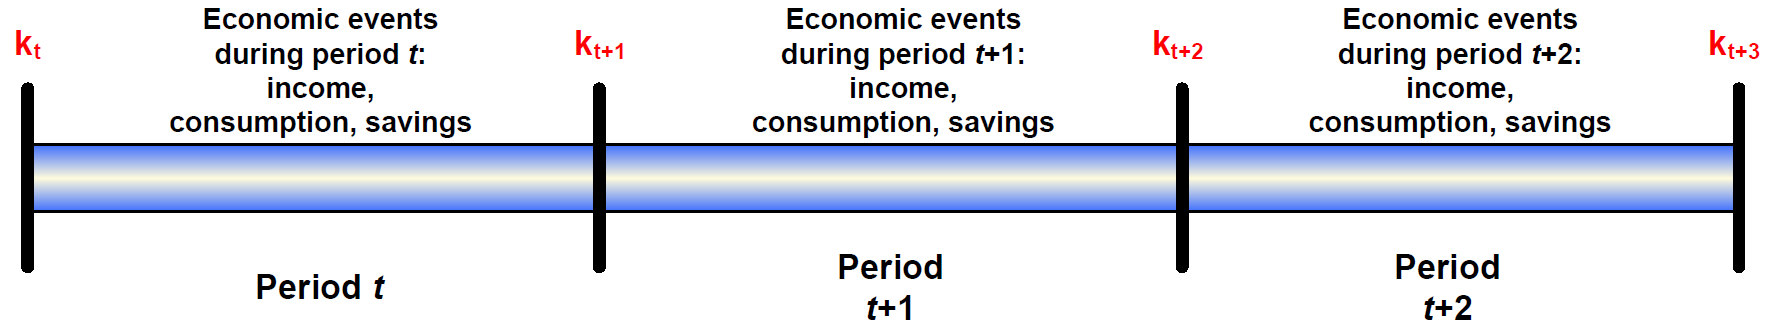
\includegraphics[trim=0 0 0 0,clip,width=1.1\textwidth]{FIGURES/10_Time_cropped}
	}      
	%\subfigure{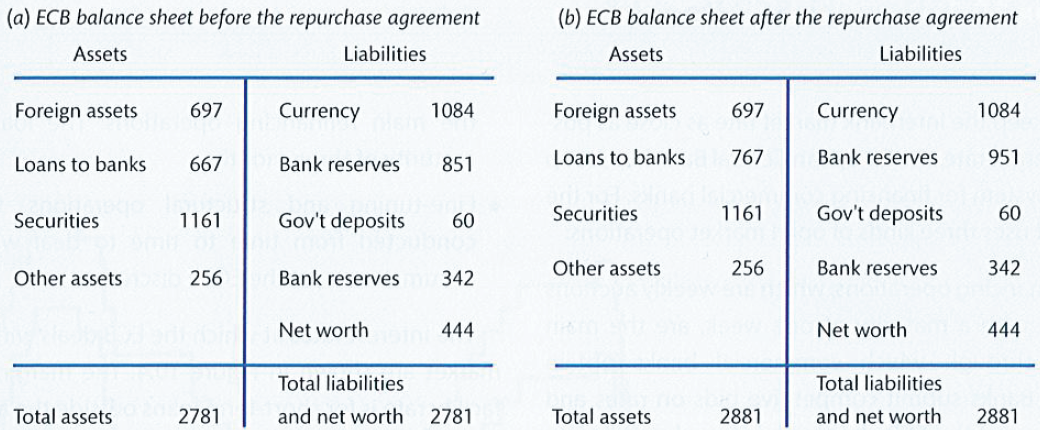
\includegraphics[trim=0 00 0 00,clip,width=0.6\textwidth]{FIGURES/5_CB_balance_sheet_OMO}
	%} 	
	%[trim=left bottom right top
\end{figure}
%\vspace{-2mm}
%\begin{minipage}{0.5\columnwidth}
%\tiny	
%\textbf{Source.} Burda and Wyplosz (2017), Figure 14.1.\\
%\end{minipage}
\end{center}
\end{frame}


\begin{frame}{Law of motion of productivity}
  Productivity is stochastic (random), but has some persistence: it follows a stochastic autoregressive process of order 1 (in logs):
  \vfill
  \begin{align*}
	\ln Z_t = \rho \ln Z_{t-1} + \epsilon_t, \quad \epsilon_t \sim \mathcal N(0, \sigma^2_\epsilon) 
  \end{align*}
  where $\epsilon$ is the white noise component of the autoregressiove process -- the source of randomness in $Z_t$.
  \vfill
  Productivity of period $t$ is observed at $t-1$ (same timing as the capital variable)-- before the firm hires and installs capital.
\end{frame}

\begin{frame}{Law of motion of capital}
  Capital lasts for more than one period. It partially depreciates and is increased by \tb{investment}: 
  \vfill
  \begin{align*}
	K_{t+1} &= K_{t} \underbrace{- \delta K_t}_{\text{depreciation}} + I_t \\
	&= (1-\delta) K_t + I_t
  \end{align*}
  \vfill
  Closed economy \rarr investment is financed only with households' \tb{savings}
\end{frame}

\begin{frame}{Building the Equilibrium}
  \tm{Capital market clearing} \\
  \begin{mytemize}
  \item Capital demand from firm's profit maximization: $K_{t+1} = K^d(r_t)$
  \item Capital supply is savings supply: $I_t = \underbrace{\Omega_{t+1} - \Omega_t}_{=G(r_t)}$ 
  \item Combining with law of motion of capital: 
	\begin{equation*}
	  K^d(r_t) = (1-\delta)K_t + G(r_t)
	\end{equation*}
  \end{mytemize}
\vfill
\tm{Goods-market clearing}
\begin{mytemize}
\item Goods aggregate supply is $Y_t$, given by $Z_t f(K_t,L_t)$
\item Goods aggregate demand is $C_t+I_t \ \ (= C_t + K_{t+1} - (1-\delta)K_t)$ 
\item Goods market clearing
\begin{align*}
  C_t+K_{t+1}-(1-\delta)K_t=Z_t f(K_t,L_t)
\end{align*}
\item[\rarr] \tb{aggregate resource constraint}
\end{mytemize}
\vfill
\tm{Labor market clearing}
\begin{align*}
  L^s(w_t, C_t) = L^d(w_t)
\end{align*}
\end{frame}
%---FRAME------------------------------------------------------------------------------
%\begin{frame}{"Sequence of markets" equilibrium}
%
%\begin{mytemize}
%\small
%\item Have determined the \emph{market clearing conditions} in terms of \tb{quantities}
%\item The prices that clear period $t$ markets are
%\begin{mytemize}
%\small
%\item $w_t$ (labour market)
%\item $r_t$ (capital market)
%\item $1$ (goods market - numeraire market)
%\end{mytemize}
%\item Have been focusing on period $t$ equilibrium
%\item But original problem specified the conditional time-zero information
%\item $\Rightarrow$ a "sequence of markets" equilibrium definition
%\end{mytemize}
%\small
%
%
%\end{frame}
%%---FRAME------------------------------------------------------------------------------
%\begin{frame}{Definition: Competitive equilibrium}
%
%A competitive equilibrium is a sequence $\left\{ C_t,L_t, K_{t+1},w_t\right\}_{t=0}^{\infty}$ that, given $K_0$ and the exogenous stochastic processes, satisfies the following:
%\begin{enumerate}
%\small
%\item Given $\left\{ r_t,w_t\right\}_{t=0}^{\infty}$, $\left\{ C_t, L_t,K_{t+1}\right\}_{t=0}^{\infty}$ satisfies the sequence of C-L optimality conditions, C-S optimality conditions, and consumer flow budget constraints
%\item Given $\left\{r_t, w_t \right\}_{t=0}^{\infty}$, $\left\{ L_t,K_t\right\}_{t=0}^{\infty}$ satisfies the sequence of labour demad functions and capital demand functions
%\item Markets clear: $C_t+K_{t+1}-(1-\delta)K_t=Z_t f(K_t,L_t)=y$; $L^s_t=L^d_t=L_t$; $k^s_t=k^d_t=K_t$
%\end{enumerate}
%
%\end{frame}
%%---FRAME------------------------------------------------------------------------------
%\begin{frame}{Competitive equilibrium}
%
%{
%\small
%A competitive equilibrium is a sequence $\left\{C_t,L_t,K_{t+1},r_t, w_t \right\}_{t=0}^{\infty}$ that, given $K_0$ and the exogenous stochastic processes, satisfies
%\begin{align*}
%\frac{u_n(C_t,1-L_t)}{u_c(C_t,1-L_t)}=& w_t \nonumber\\
%1 =& E_t \left[ \left( \frac{\beta \lambda_{t+1}}{\lambda_t}\right)(1+r_{t+1}-\delta)\right] \nonumber\\
% Z_t f_n(K_t,L_t)-w_t =& 0 \nonumber\\
% Z_t f_k(K_t,L_t)-r_t =& 0 \nonumber\\
%C_t+K_{t+1}-(1-\delta)K_t=& Z_t f(K_t,L_t) \nonumber
%\end{align*}
%(consumption-leisure, consumption-savings/Euler eq., labour demand, capital demand, aggr. resource constraint) \tb{for t=0,1,2,...}.
%
%\smallskip
%\tb{Further issues \& discussion}
%}
%\begin{mytemize}
%\footnotesize
%\item Note: Euler equation is a difference equation
%\item Firm profits in equilibrium: $\Pi_t=Z_t f(K_t,L_t)-w_tL_t-r_t K_t$
%\item Also need a terminal condition for the difference system - \tb{transversality condition}
%\end{mytemize}
%
%\end{frame}
%%---FRAME------------------------------------------------------------------------------
%\begin{frame}{Transversality condition}
%
%\begin{mytemize}
%\small
%\item Transversality condition (TVC) needed because difference system is of \alert{second-order in the capital stock $k$}
%\item $\rightarrow$ two endpoint conditions required: $K_0$ and TVC
%\item Successive forward substitution for $k$ terms in the flow budget constraint leads to 
%\end{mytemize}
%
%\begin{align*}
%K_0 = \sum_{s=0}^{\infty} \left( \frac{C_s-w_sL_s-\prod_s}{\prod_{\tau=0}^s(1+r_{\tau}-\delta)}\right)+\underbrace{\lim_{T\rightarrow \infty}\frac{K_{T}}{\prod_{\tau=0}^{T}(1+r_{\tau}-\delta)}}_{\lim=0}
%\end{align*}
%
%\begin{mytemize}
%\small
%\item \emph{Interpretation:} value of initial of assets = PDV of all future dissavings consumer will engage in, plus PDV of assets at end of planning horizon (should be zero=TVC!)
%\item No Ponzi Game condition
%\item (We will ignore this moving forward.)
%\end{mytemize}
%
%
%\end{frame}
%%---FRAME------------------------------------------------------------------------------
%\begin{frame}{Equilibrium - compact}
%
%{
%\small
%A competitive equilibrium is a sequence $\left\{C_t,L_t,K_{t+1},r_t, w_t \right\}_{t=0}^{\infty}$ that, given $K_0$ and the exogenous stochastic processes, satisfies
%\begin{align*}
%\frac{u_n(C_t,1-L_t)}{u_c(C_t,1-L_t)}=& Z_t f_n(K_t,L_t) \nonumber\\
%1 =& E_t \left[ \left( \frac{\beta \lambda_{t+1}}{\lambda_t}\right)(1+Z_{t+1} f_k(K_{t+1},L_{t+1})-\delta)\right] \nonumber\\
%C_t+K_{t+1}-(1-\delta)K_t=& Z_t f(K_t,L_t) \nonumber
%\end{align*}
%
%\begin{mytemize}
%\item In practice, solve (computationally) the equilibrium
%\item Is there a simpler problem that gives the same solution? (\emph{if perfect equilibrium, yes...})
%\end{mytemize}
%
%}
%\end{frame}
%%---FRAME------------------------------------------------------------------------------
%%---FRAME------------------------------------------------------------------------------
%\subsection{Planning Problem}
%%---FRAME------------------------------------------------------------------------------
%\begin{frame}
%\frametitle{Outline}
%\tableofcontents[currentsubsection]
%\end{frame}
%%---FRAME------------------------------------------------------------------------------
%\begin{frame}{Planning Problem}
%
%\begin{mytemize}
%\small
%\item The Social Planner
%\begin{mytemize}
%\small
%\item A fictional device useful for deriving efficient outcomes as a result
%\item A "benevolent central planner" for an economy \\
%$\rightarrow$ maximizes welfare (utility) of representative consumer (\emph{benevolent})
%\item Powerful: can simply order/command/direct/shift around costlessly the productive resources of an economy
%\end{mytemize}
%\item Conceptual implementation of a Social Planner problem
%\begin{mytemize}
%\footnotesize
%\item Social Planner does not need/does not take account of any market forces or prices
%\item Only cares about primitives of the economy
%\item Basic RBC model: primitives are consumers' preferences and production technology available to convert inputs into outputs
%\end{mytemize}
%\item Mathematical implementation of a Social Planner problem
%\begin{mytemize}
%\footnotesize
%\item Maximize utility...
%\item ...subject to relevant resource constraint(s)
%\item i.e., not subject to any 'budget constraints' or 'prices' germane to private-sector consumers and firms
%\end{mytemize}
%\end{mytemize}
%
%
%\end{frame}
%%---FRAME------------------------------------------------------------------------------
%\begin{frame}{Social Planner Optimization}
%
%
%{
%\small
%\begin{align*}
%\max_{\left\{ C_t, L_t, K_{t+1} \right\}} E_0 \sum_{t=0}^{\infty} \beta^t  u(C_t,1-L_t)
%\end{align*}
%s.t. a \emph{sequence} of \tb{resource} constraints
%\begin{align*}
%C_t + K_{t+1}-(1-\delta)K_t = Z_t f(K_t,L_t) \quad \text{for each } t=0,1,2,...
%\end{align*}
%}
%\begin{mytemize}
%\footnotesize
%\item Put up the Lagrangian with multiplier $\rho_t$
%\item Social Planner takes as given
%\begin{mytemize}
%\footnotesize
%\item $K_0$ - a stock variable (initial condition)
%\item stochastic process for TFP
%\end{mytemize}
%\end{mytemize}
%
%{
%\small
%FOCs:
%\begin{align*}
%&(1) \quad \frac{\partial \mathcal{L}}{C_t}: \quad & & u_c(C_t,1-L_t)-\rho_t = 0\\
%&(2) \quad \frac{\partial \mathcal{L}}{L_t}: \quad &  &-u_n(C_t,1-L_t)+\rho_t Z_t f_n(K_t,L_t)=0\\
%&(3) \quad \frac{\partial \mathcal{L}}{K_{t+1}}: \quad &  &-\rho_t  +\beta E_t[\rho_{t+1}(1+Z_{t+1}f_k(K_{t+1},L_{t+1})-\delta)]=0 \\
%\end{align*}
%}
%
%\end{frame}
%%---FRAME------------------------------------------------------------------------------
%\begin{frame}{Efficient allocations}
%
%Efficient allocations are given by the conditions
%\begin{align*}
%\frac{u_n(C_t,1-L_t)}{u_c(C_t,1-L_t)}=& Z_t f_n(K_t,L_t) \nonumber\\
%1 =& E_t \left[ \left( \frac{\beta \rho_{t+1}}{\rho_t}\right)(1+Z_{t+1} f_k(K_{t+1},L_{t+1})-\delta)\right] \nonumber\\
%C_t+K_{t+1}-(1-\delta)K_t=& Z_t f(K_t,L_t) \nonumber
%\end{align*}
%...which are \tb{identical to the competitive equilibrium} case!
%
%\end{frame}
%%---FRAME------------------------------------------------------------------------------
%\begin{frame}{Welfare Theorems}
%
%\begin{mytemize}
%\small
%\item \tb{First Welfare Theorem:} any competitive equilibrium leads to a Pareto efficient allocation (i.e. the planner cannot make one person better off without making another person worse off.)
%\begin{mytemize}
%\footnotesize
%\item Perfect competition (price-takers)
%\item full information/ no externalities
%\end{mytemize}
%\item Makes computing solution easier
%\begin{mytemize}
%\footnotesize
%\item but with advances in computing power, becomes actually not a constraint
%\end{mytemize}
%\item Non-lump sum taxes break the equivalence - (e.g. proportional taxes on labour income and capital income)
%\item Need to work directly with equilibrium conditions if want to consider taxes.
%\end{mytemize}
%
%\end{frame}
%%---FRAME------------------------------------------------------------------------------
%\begin{frame}{Summary: Why Microfoundations?}
%
%\begin{mytemize}
%\small
%\item Consumer preferences
%\item Production technologies
%\begin{mytemize}
%\small
%\item Operated by firms
%\item but industrial organization not specified
%\end{mytemize}
%\item Perfect competition $\leftrightarrow$ can work with Social Planner problem
%\item Next: a quantitative assessment
%\begin{mytemize}
%\item calibration
%\item simulation
%\item comparison with data and IRFs
%\end{mytemize}
%\end{mytemize}
%
%\end{frame}
%---FRAME------------------------------------------------------------------------------
%---FRAME------------------------------------------------------------------------------
%---FRAME------------------------------------------------------------------------------
%---FRAME------------------------------------------------------------------------------
%\section{Solution and quantitative assessment}
%%---FRAME------------------------------------------------------------------------------
%\begin{frame}
%\frametitle{Outline}
%\tableofcontents[currentsection]
%\end{frame}
%%---FRAME------------------------------------------------------------------------------
%\begin{frame}{How to use the model?}
%
%Necessary steps:
%\begin{enumerate}
%\small
%\item Choose functional forms
%\item Pick values for model parameters $[\delta,\alpha,\theta,\eta,\gamma,\rho,\sigma]$
%\item Compute the steady state of the model
%\item Compute a linear approximation to the non-linear equilibrium conditions
%\item Solve the model
%\item Use the linear solution for quantitative assessment
%\end{enumerate}
%
%\end{frame}
%%---FRAME------------------------------------------------------------------------------
%\subsection{Functional forms}
%%---FRAME------------------------------------------------------------------------------
%\begin{frame}
%\frametitle{Outline}
%\tableofcontents[currentsubsection]
%\end{frame}
%%---FRAME------------------------------------------------------------------------------
%\begin{frame}{Functional forms}
%
%\begin{mytemize}
%\small
%\item \tb{Technology shocks}
%\begin{align*}
%ln Z_t = \rho ln Z_{t-1} + \varepsilon_t
%\end{align*} 
%with $\rho \in (0,1)$ and $\varepsilon_t \sim \mathcal{N}(0,\sigma)$
%\item $Z_t$ is the only exogenous variable in the model
%\item $\alert{\rho}$ serial correlation, $\alert{\sigma}$ variance of shock
%\item \tb{Preferences}
%\begin{align*}
%\frac{C_t^{1-\gamma}}{{1-\gamma}} + \theta \frac{(1-L_t)^{1-\eta}}{1-\eta},
%\end{align*}
%where $\gamma$ is the coefficient of relative risk aversion, $\eta$ is the marginal disutility of labour supply, $\theta$ is a weight on leisure to determine quantities in equilibrium.
%\item \tb{Production function}
%\begin{align*}
%y_t = Z_t K_t^{\alpha}L_t^{1-\alpha},
%\end{align*}
%with $\alpha$ being the capital share (note parallel with neoclassical growth model).
%\end{mytemize}
%
%\end{frame}
%%---FRAME------------------------------------------------------------------------------
%\begin{frame}{Common utility functions}
%
%\begin{mytemize}
%\small
%\item Constant relative risk aversion (CRRA)
%\begin{align*}
%u(C_t,1-L_t)=\frac{C_t^{1-\gamma}}{{1-\gamma}} + \theta \frac{(1-L_t)^{1-\eta}}{1-\eta},
%\end{align*}
%\begin{mytemize}
%\small
%\item Arrow-Pratt measures of risk aversion $(-cu''(c)/u'(c))$
%\item \textit{Examples:} Gali 2008, Gali and Monacelli 2005, Ravenna and Walsh 2006.
%\end{mytemize}
%\item Logarithmic utility
%\begin{align*}
%u(C_t,1-L_t)=ln(C_t) + \frac{L_t}{L_0} A ln(1-L_0)
%\end{align*}
%\begin{mytemize}
%\small
%\item Limiting case for $\gamma \rightarrow 1$
%\item \emph{Example:} Hansen 1985
%\end{mytemize}
%
%\item Combination of logarithmic and CRRA
%\begin{align*}
%u(C_t,1-L_t)= ln(C_t) - \frac{\nu}{1+\chi} L_t^{1+\chi}
%\end{align*}
%\emph{Example:} Gertler and Karadi 2011
%\end{mytemize}
%
%% check also: 
%%% - Greenwood-Hercowitz-Huffan preferences
%%% - King-Plosser-Rebelo preferences
%%% - Jaimovich-Rebelo preferences
%%% - Epstein-Zin preferences
%
%
%\end{frame}
%%---FRAME------------------------------------------------------------------------------
%\begin{frame}{Equations and variables}
%
%{
%\footnotesize
%
%HH's labor-leisure decision
%\begin{align*}
%\frac{\theta(1-L_t)^{-\eta}}{C_t^{-\gamma}}=w_t 
%\end{align*}
%
%Euler equation
%\begin{align*}
%1 =  E_t \left[\frac{\beta C_{t+1}^{-\gamma}}{C_t^{-\gamma}}(1+r_{t+1}-\delta)\right]
%\end{align*}
%
%Firms capital demand
%\begin{align*}
%\alpha Z_tK_t^(\alpha-1)L_t^(1-\alpha)= r_t
%\end{align*}
%
%
%Firms labor demand
% \begin{align*}
%(1-\alpha)Z_tK_t^{\alpha}L_t^{-\alpha} = w_t
% \end{align*}
%
%
%Resource constraint
%\begin{align*}
%w_tL_t+r_tK_t+(1-\delta)K_t = C_t+K_{t+1};
%\end{align*}
%
%
%Output
%\begin{align*}
%y_t = Z_tK_t^{\alpha}L_t^{(1-\alpha)};
%\end{align*} 
%
%
%Law of motion for productivity
%\begin{align*}
%log(Z_t) = \rho_z  log(z{t-1}) + \epsilon_t;
%\end{align*}
%
%
%}
%
%\end{frame}
%
%%---FRAME------------------------------------------------------------------------------
%\begin{frame}{Equations and variables (cont'd)}
%
%\begin{mytemize}
%\item 7 equations in the unknowns
%\item exgenous: $Z_t$
%\item endogenous: $C_t$, $L_t$, $K_{t+1}$
%\item ...then, easy to express $w_t$, $r_t$, $y_t$ as functions of $Z_t$, $L_t$ and $K_t$
%\item Need to specify/solve for functions ('decision rules') that describe how:
%\begin{mytemize}
%\item comsumers make choices based on prices and policies
%\item firms make choices based on prices and policies
%\item prices depend on state variables (capital, TFP)
%\end{mytemize}
%\item $\rightarrow$ turn to quantitative/numerical methods
%\item because of \alert{second-order difference system} (consumption-savings optimiality condition is a a \emph{second-order difference equation} in $K_t$)
%\end{mytemize}
%
%
%\end{frame}
%%---FRAME------------------------------------------------------------------------------
%\subsection{Calibration}
%%---FRAME------------------------------------------------------------------------------
%\begin{frame}
%\frametitle{Outline}
%\tableofcontents[currentsubsection]
%\end{frame}
%%---FRAME------------------------------------------------------------------------------
%\begin{frame}{Calibration}
%
%\begin{center}
%
%\begin{tabular}{c c c c c c c c}
%\toprule
%$\beta$ & $\alpha$ & $\eta$ & $\gamma$ & $\delta$ & $\theta$ & $\rho$ & $\sigma_z$ \\ 
%\hline 
%0.984 & 0.33 & 1 & 2 & 0.025 & 7.37 & 0.979 & 0.0072 \\ 
%\bottomrule
%\end{tabular} 
%\end{center}
%
%\vspace{3mm}
%{
%\small
%Following King \& Rebelo (1999) }
%\begin{mytemize}
%\small
%\item Choose discount factor $\beta$ to yield interest rate of $6.5\%$ per annum (avg $S\&P500$ 1948-1986), thus $\bar{r}=0.065/4$
%\item Cobb-Douglas PF: Set $\alpha=1/3$
%\item Capital depreciation rate is 10\% per annum $(\delta=0.1/4=0.025)$
%\item $\theta$ is a scaling parameter to match steady state labor $\bar{n}$ to represent $20\%$ of the available time.
%\item Frisch elasticity $(1/\eta)$ is the elasticity of labor supply with respect to the wage, keeping marginal utility of wealth constant. It measures the \emph{substitution effect}.
%\item The coefficient of risk aversion is calibrated to 2 (in contrast with King and Plosser who use log utility in consumption, thus $\gamma=1$)
%\end{mytemize}
%
%\end{frame}
%%---FRAME------------------------------------------------------------------------------
%\subsection{Steady state}
%\begin{frame}
%\frametitle{Outline}
%\tableofcontents[currentsubsection]
%\end{frame}
%%---FRAME------------------------------------------------------------------------------
%\begin{frame}{Steady state}
%
%\begin{mytemize}
%\small
%\item Steady state, situation in which $\bar{z}=1$,
%\item Thus generally: $E_t(x_{t+1})=x_t=x_{t-1}=x_{ss} \equiv \bar{x}$
%\item $K_{t+1}=K_t=\bar{k}$, and $C_{t+1}=C_t=\bar{c}$
%\item then, we can back out steady state values of static variables ($\bar{w},\bar{n},\bar{r}...$)
%\end{mytemize}
%{
%\small
%Start with optimal capital input of firms to define the capital-labor ratio as
%\begin{align*}
%\frac{\bar{k}}{\bar{n}} = \left(\frac{\bar{r}}{\bar{z} \alpha} \right)^{\frac{1}{\alpha-1}}
%\end{align*}
%combine with the steady state Euler equation
%\begin{align*}
%\bar{r} = \frac{1}{\beta}-1+\delta
%\end{align*}
%}
%\end{frame}
%%---FRAME------------------------------------------------------------------------------
%\begin{frame}{Steady state (cont'd)}
%
%\begin{mytemize}
%\small
%\item Next, use the calibration target $\bar{n}=0.2$ 
%\begin{align*}
%\bar{k}=\frac{\bar{k}}{\bar{n}} \bar{n}
%\end{align*}
%and finally, using the aggregate resource constraint
%\begin{align*}
%\bar{c}= \left[  \left( \frac{\bar{k}}{\bar{n}}\right)^{\alpha}  -\delta \left(\frac{\bar{k}}{\bar{n}} \right)  \right] \bar{n}
%\end{align*}
%\item The endogenous scaling parameter $\theta$ takes then the value (from the HH's intra-temporal decision)
%\begin{align*}
%&\theta = -\frac{\bar{w}\bar{c}^{-\gamma}}{(1-\bar{n})^{-\eta}}, \\
%\textnormal{where } &\bar{w} = (1-\alpha) \frac{\bar{k}}{\bar{n}}
%\end{align*}
%\end{mytemize}
%\end{frame}
%%---FRAME------------------------------------------------------------------------------
%\subsection{Solution methods}
%%---FRAME------------------------------------------------------------------------------
%\begin{frame}
%\frametitle{Outline}
%\tableofcontents[currentsubsection]
%\end{frame}
%%---FRAME------------------------------------------------------------------------------
%\begin{frame}{Solution methods}
%
%{
%\small
%\begin{mytemize}
%\item Looking for an equilibrium in which endogenous variables are functions of the \tb{state} of the model, $S_t=[K_t,Z_t]$
%\begin{mytemize}
%\item State describes the 'position' of the model
%\item So looking for $c(S_t),n(S_t),k(S_t)$
%\item Markov/AR(p) assumption is critical here.
%\end{mytemize}
%\item Cannot solve difference equations analytically in general
%\begin{mytemize}
%\item ... solutions are \emph{unknowable} in general
%\item Hence, need to approximate: $c^{approx}(S_t), L^{approx}(S_t),k^{approx}(S_t)$, which are hopefully near the truth.
%\end{mytemize}
%\end{mytemize}
%}
%
%\end{frame}
%%---FRAME------------------------------------------------------------------------------
%\begin{frame}{The general problem}{System of second-order difference equations}
%
%Deterministic, perfect foresight, case:
%\[
%f(y_{t+1},y_t,y_{t-1},u_t)=0
%\]
%Stochastic case:
%\[
%\mathbb{E}_t\left\{f(y_{t+1},y_t,y_{t-1},u_t)\right\}=0
%\]
%\begin{mytemize}
%  \item[$y$]: vector of endogenous variables
%  \item[$u$]: vector of exogenous shocks
%\end{mytemize}
%
%$\Rightarrow$ The software DYNARE provides solutions to such problems.
%\end{frame}
%%---FRAME------------------------------------------------------------------------------
%\begin{frame}{Approximations}
%
%{
%\small
%\tb{Global:} approximated functions are close to the true functions \emph{everywhere} (i.e. over a broader range of states) 
%\begin{mytemize}
%\item Hard to implement for medium- and large-scale models given current hardware capacity
%\item Several popular methods:
%\begin{mytemize}
%\item Chebyshev polynomials
%\item Finite-element methods
%\item Value function iteration
%\end{mytemize}
%\end{mytemize}
%
%\tb{Local:} approximated functions are close to true functions only in a relatively small range of states
%\begin{mytemize}
%\item Much easier to implement
%\item All based on Taylor approximations
%\begin{mytemize}
%\item Linear (first-order)
%\item Quadratic (second-order)
%\item etc.
%\end{mytemize}
%\end{mytemize}
%}
%
%\end{frame}
%%---FRAME------------------------------------------------------------------------------
%\begin{frame}{Approximations}
%
%\begin{figure}[h!]
%%\caption{Figure. Net}
%	\subfigure{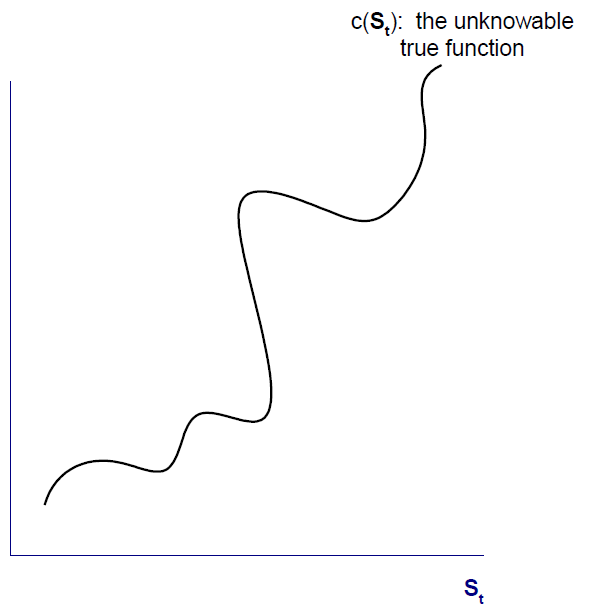
\includegraphics[trim=0 0 0 0,clip,width=0.7\textwidth]{FIGURES/10_RBCapprox1}
%	}      
%	%} 		
%%	\label{fig:GPD} 
%	%[trim=left bottom right top
%\end{figure}
%
%\end{frame}
%%---FRAME------------------------------------------------------------------------------
%\begin{frame}{Approximations}
%
%\begin{figure}[h!]
%%\caption{Figure. Net}
%	\subfigure{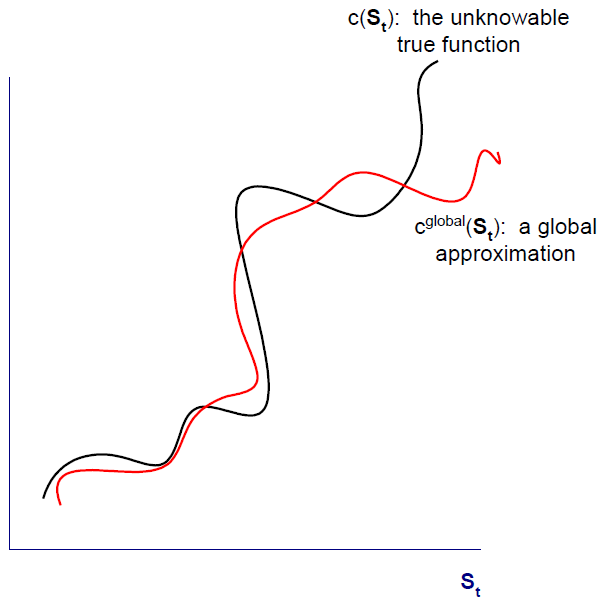
\includegraphics[trim=0 0 0 0,clip,width=0.7\textwidth]{FIGURES/10_RBCapprox2}
%	}      
%	%} 		
%%	\label{fig:GPD} 
%	%[trim=left bottom right top
%\end{figure}
%
%\end{frame}
%%---FRAME------------------------------------------------------------------------------
%\begin{frame}{Approximations}
%
%\begin{figure}[h!]
%%\caption{Figure. Net}
%	\subfigure{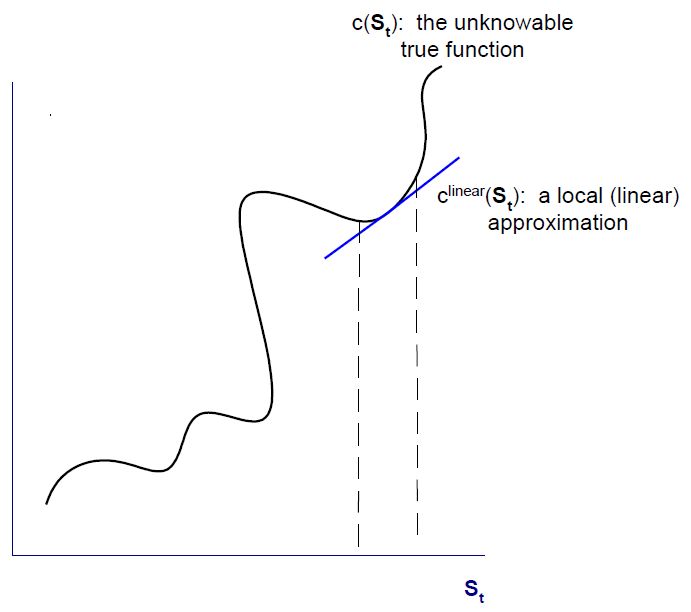
\includegraphics[trim=0 0 0 0,clip,width=0.7\textwidth]{FIGURES/10_RBCapprox3}
%	}      
%	%} 		
%%	\label{fig:GPD} 
%	%[trim=left bottom right top
%\end{figure}
%
%\end{frame}
%%---FRAME------------------------------------------------------------------------------
%\begin{frame}{Approximations}
%
%\begin{figure}[h!]
%%\caption{Figure. Net}
%	\subfigure{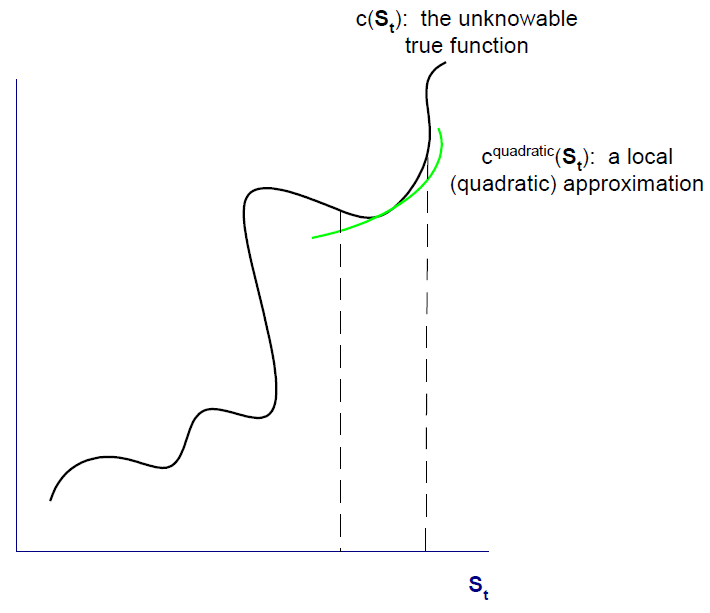
\includegraphics[trim=0 0 0 0,clip,width=0.7\textwidth]{FIGURES/10_RBCapprox4}
%	}      
%	%} 		
%%	\label{fig:GPD} 
%	%[trim=left bottom right top
%\end{figure}
%
%\end{frame}
%%---FRAME------------------------------------------------------------------------------
%\begin{frame}{Approximations}
%
%\begin{figure}[h!]
%%\caption{Figure. Net}
%	\subfigure{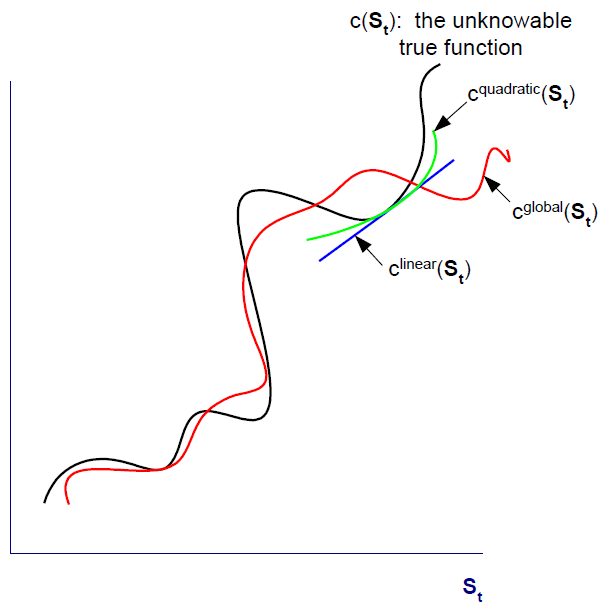
\includegraphics[trim=0 0 0 0,clip,width=0.7\textwidth]{FIGURES/10_RBCapprox5}
%	}      
%	%} 		
%%	\label{fig:GPD} 
%	%[trim=left bottom right top
%\end{figure}
%
%\end{frame}
%%---FRAME------------------------------------------------------------------------------
%\begin{frame}{Approximations}
%
%\begin{figure}[h!]
%%\caption{Figure. Net}
%	\subfigure{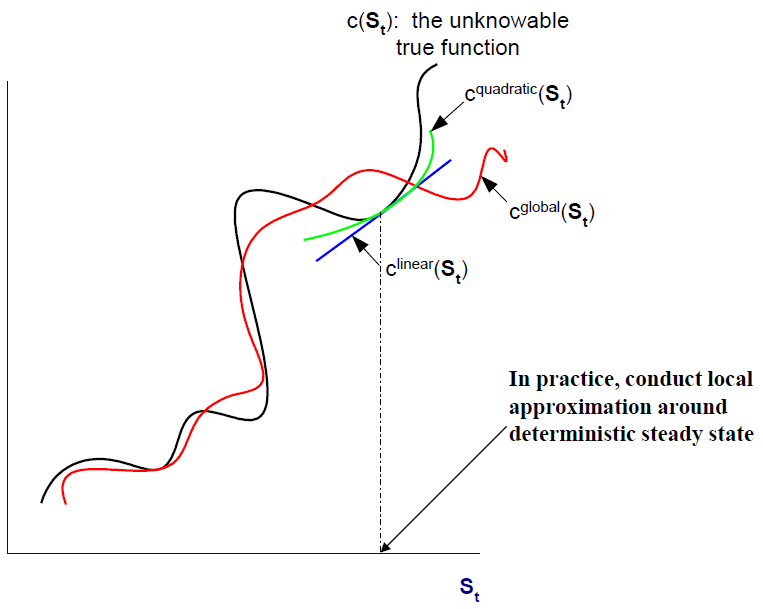
\includegraphics[trim=0 0 0 0,clip,width=0.7\textwidth]{FIGURES/10_RBCapprox6}
%	}      
%	%} 		
%%	\label{fig:GPD} 
%	%[trim=left bottom right top
%\end{figure}
%
%\end{frame}
%%---FRAME------------------------------------------------------------------------------
%\begin{frame}{Example: First order approximation for stochastic models in dynare}
%
%\begin{mytemize}
%  \item Perturbation approach: recovering a Taylor expansion of the solution function from a Taylor expansion of the original model.
%  \item A first order approximation is nothing else than a standard solution through linearization.
%  \item A first order approximation in terms of the logarithm of the variables provides standard log-linearization.
%  \end{mytemize}
%
%\end{frame}
%%---FRAME------------------------------------------------------------------------------
%\begin{frame}{General model}
%
%\[
%\mathbb{E}_t\left\{f(y_{t+1},y_t,y_{t-1},u_t)\right\}=0
%\]
%\begin{eqnarray*}
%\mathbb{E}(u_t) &=& 0\\
%\mathbb{E}(u_tu_t') &=& \Sigma_u\\
%\mathbb{E}(u_tu_\tau') &=& 0\;\;\;\;t\ne\tau
%\end{eqnarray*}
%
%\begin{mytemize}
%  \item[$y$]: vector of endogenous variables
%  \item[$u$]: vector of exogenous stochastic shocks
%\end{mytemize}
%
%\end{frame}
%%---FRAME------------------------------------------------------------------------------
%\begin{frame}{Timing assumptions}
%
% \[
%  \mathbb{E}_t\left\{f(y_{t+1},y_t,y_{t-1},u_t)\right\}=0
%  \]
%  \begin{mytemize}
%  \item shocks $u_t$ are observed at the beginning of period $t$,
%  \item decisions affecting the current value of the variables $y_t$, are function of
%    \begin{mytemize}
%    \item the previous state of the system, $y_{t-1}$,
%    \item the shocks $u_t$.
%    \end{mytemize}
%  \end{mytemize}
%  
%\end{frame}
%%---FRAME------------------------------------------------------------------------------
%\begin{frame}{The stochastic scale variable}
%
%\[
%\mathbb{E}_t\left\{f(y_{t+1},y_t,y_{t-1},u_t)\right\}=0
%\]
%\begin{mytemize}
%\item At period $t$, the only unknown stochastic variable is $y_{t+1}$, and, implicitly, $u_{t+1}$.
%\item We introduce the \emph{stochastic scale variable}, $\sigma$ and the auxiliary random variable, $\epsilon_t$, such that
%\[
%u_{t+1} = \sigma\epsilon_{t+1}
%\]
%\end{mytemize}
%
%\end{frame}
%%---FRAME------------------------------------------------------------------------------
%\begin{frame}{The stochastic scale variable (continued)}
%
%\begin{align}
%\mathbb{E}(\epsilon_t) &= 0\\
%\mathbb{E}(\epsilon_t\epsilon_t') &= \Sigma_\epsilon\\
%\mathbb{E}(\epsilon_t\epsilon_\tau') &= 0\;\;\;\;t\ne\tau  
%\end{align}
%and
%\[
%\Sigma_u = \sigma^2\Sigma_\epsilon
%\]
%
%\end{frame}
%%---FRAME------------------------------------------------------------------------------
%\begin{frame}{Remarks}
%
%\[
%\mathbb{E}_t\left\{f(y_{t+1},y_t,y_{t-1},u_t)\right\}=0
%\]
%  \begin{mytemize}
%  \item The exogenous shocks may appear only at the current period
%  \item There is no deterministic exogenous variables
%  \item Not all variables are necessarily present with a lead and a lag
%  \item Dynare transforms models with leads and lags on more than one
%    period in an equivalent model with leads and lags on one period
%    with the addition of auxiliary endogenous variables. Special care
%    is taken to preserve expectation of non-linear functions.
%  \end{mytemize}
%
%\end{frame}
%%---FRAME------------------------------------------------------------------------------
%\begin{frame}{Solution function}
%
%\[
%y_t = g(y_{t-1},u_t,\sigma)
%\]
%where $\sigma$ is the stochastic scale of the model. If $\sigma = 0$, the model is deterministic. For $\sigma > 0$, the model is stochastic.
%
%\medskip
%
%Under some conditions, the existence of $g()$ function is proven via an implicit function theorem. See H. Jin and K. Judd ``Solving Dynamic Stochastic Models'' {\tiny (\url{http://bucky.stanford.edu/papers/PerturbationMethodRatEx.pdf})}
%
%\end{frame}
%%---FRAME------------------------------------------------------------------------------
%\begin{frame}{Solution function (continued)}
%
%Then,
%
%\begin{align*}
%  y_{t+1} =& g(y_t,u_{t+1},\sigma)\\
%  =& g(g(y_{t-1},u_t,\sigma),u_{t+1},\sigma)\\
%\lefteqn{F(y_{t-1},u_t,\epsilon_{t+1},\sigma)}\\
% =& f(g(g(y_{t-1},u_t,\sigma),\sigma\epsilon_{t+1},\sigma),g(y_{t-1},u_t,\sigma),y_{t-1},u_t)
%\end{align*}
%
%\begin{align*}
%  \mathbb{E}_t\left\{F(y_{t-1},u_t,\alert{ \epsilon_{t+1}},\sigma)\right\} = 0
%\end{align*}
%
%\end{frame}
%%---FRAME------------------------------------------------------------------------------
%\begin{frame}{The perturbation approach}
%
%\begin{mytemize}
%  \item Obtain a Taylor expansion of the unknown solution function in the neighborhood of a problem that we know how to solve.
%  \item The problem that we know how to solve is the deterministic steady state.
%  \item One obtains the Taylor expansion of the solution for the Taylor expansion of the original problem.
%  \item One consider two different perturbations:
%    \begin{enumerate}
%    \item points in the neighborhood from the steady sate,
%    \item from a deterministic model towards a stochastic one (by increasing $\sigma$ from a zero value).
%    \end{enumerate}
%  \end{mytemize}
%
%\end{frame}
%%---FRAME------------------------------------------------------------------------------
%\begin{frame}{Taylor expansion}
%
% Univariate, $y=g(x)$,
%\[
%y \approx g(x_0) + \sum_{k=1}^\infty
%\frac{1}{k!}\frac{d^kg}{dx^k}(x-x_0)^k
%\]
%Multivariate, $y=g(x)$, $y \in \mathbb{R}^n$, $x \in \mathbb{R}^m$,
%\[
%y \approx g(x_0) + \sum_{k=1}^\infty
%\frac{1}{k!}\frac{\partial^kg}{\partial x^k}(x-x_0)\otimes\ldots\otimes(x-x_0)
%\]
%
%\end{frame}
%%---FRAME------------------------------------------------------------------------------
%\begin{frame}{Kronecker product}
%
%\[
%  \left[
%    \begin{array}{cc}
%      a & b\\ c & d
%    \end{array}\right]
%  \otimes
%  \left[
%    \begin{array}{cc}
%      e & f\\ g & h
%    \end{array}\right]
%  =
%  \left[
%    \begin{array}{cc|cc}
%      ae & af & be & bf\\ 
%      ag & ah & bg & bh\\
%      \hline
%      ce & cf & de & df\\ 
%      cg & ch & dg & dh
%    \end{array}\right]
%  \]
%
%\end{frame}
%%---FRAME------------------------------------------------------------------------------
%\begin{frame}{The perturbation approach (continued)}
%
%\begin{mytemize}
%  \item The Taylor approximation is taken with respect to $y_{t-1}$, $u_t$ and $\sigma$, the arguments of the solution function
%    \[
%    y_t = g(y_{t-1},u_t,\sigma).
%    \]
%  \item At the deterministic steady state, all derivatives are deterministic as well.
%  \end{mytemize}
%
%\end{frame}
%%---FRAME------------------------------------------------------------------------------
%\begin{frame}{Steady state}
%
%A deterministic steady state, $\bar y$, for the model satisfies
%\[
%f(\bar y, \bar y, \bar y, 0) = 0
%\]
%A model can have several steady states, but only one of them will be used for approximation.
%
%Furthermore,
%\[
%\bar y = g(\bar y, 0, 0)
%\]
%
%\end{frame}
%%---FRAME------------------------------------------------------------------------------
%\begin{frame}{Next technical steps}
%
%\begin{enumerate}
%\item bring to structural state space representation
%\item apply generalized Schur decomposition
%\begin{mytemize}
%\item $\rightarrow$ "triangulation", upper-triangular matrix
%\item $\rightarrow$ diagonal elements are the eigenvalues of the original matrix
%\end{mytemize}
%\item select stable trajectories (existence of a unique stable trajectory)
%\begin{enumerate}
%\item there should be as many roots larger than one in modulus as there are forward-looking variables in the model (\emph{Blanchard-Kahn condition})
%\item the rank condition is verified. 
%\end{enumerate}
%\end{enumerate}
%
%\end{frame}
%%---FRAME------------------------------------------------------------------------------
%\begin{frame}{First order approximated decision function}
%
%\[
%y_t = \bar y+g_y\hat y+g_uu
%\]
%\begin{eqnarray*}
%  E\left\{y_t\right\} &=& \bar y\\
%  \Sigma_y &=& g_y \Sigma_y g_y'+\sigma^2g_u\Sigma_\epsilon g_u'
%\end{eqnarray*}
%The variance is solved for with an algorithm for Lyapunov equations.
%
%\end{frame}
%%---FRAME------------------------------------------------------------------------------
%\begin{frame}{Further resources on dynare}
%
%  \begin{mytemize}
%  \item Dynare web site: \url{http://www.dynare.org}
%  \item S. Adjemian et al. \emph{Dynare reference manual}
%  \item Dynare forum: lots of questions already answered. The first
%    place for questions.
%  \item Dynare wiki: info on bugs and Dynare development
%  \item Dynare Working Papers
%  \item Macroeconomic Model Comparison Initiative: Macroeconomic model
%    Database v.3.0: 120 published models coded in
%    Dynare (\url{http://macromodelbase.com})
%  \end{mytemize}
%  
%\end{frame}
%%---FRAME------------------------------------------------------------------------------
%\subsection{Quantitative assessment}
%%---FRAME------------------------------------------------------------------------------
%\begin{frame}
%\frametitle{Outline}
%\tableofcontents[currentsubsection]
%\end{frame}
%%---FRAME------------------------------------------------------------------------------
%\begin{frame}{Quantitative assessment}
%
%Comparing the model with the data (US data, hp-filtered)
%\medskip
%
%\begin{center}
%%{\small
%%Figure. 
%%}
%\vspace{-5mm}
%\begin{figure}[h!]
%	\subfigure{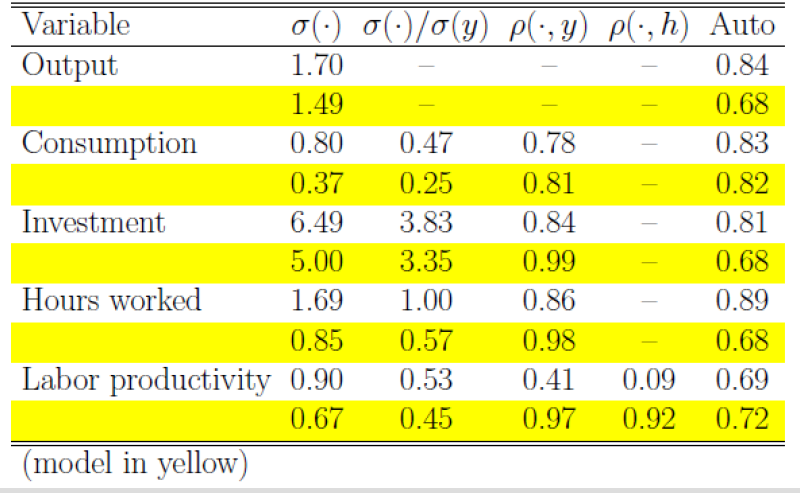
\includegraphics[trim=0 0 0 0,clip,width=0.7\textwidth]{FIGURES/10_RBCtable}
%	}      
%	%\subfigure{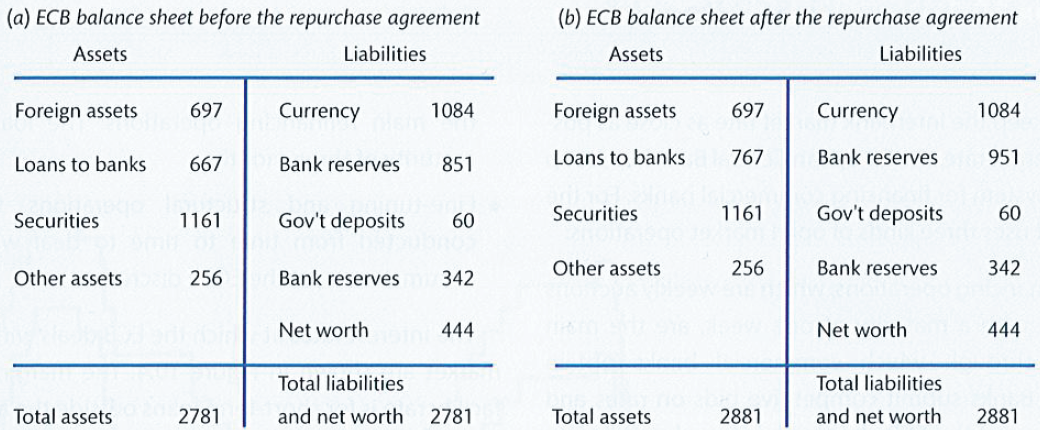
\includegraphics[trim=0 00 0 00,clip,width=0.6\textwidth]{FIGURES/5_CB_balance_sheet_OMO}
%	%} 	
%	%[trim=left bottom right top
%\end{figure}
%%\vspace{-2mm}
%%\begin{minipage}{0.5\columnwidth}
%%\tiny	
%%\textbf{Source.} Burda and Wyplosz (2017), Figure 14.1.\\
%%\end{minipage}
%\end{center}
%
%\end{frame}
%%---FRAME------------------------------------------------------------------------------
%\begin{frame}{Discussion/Summary}
%
%\begin{mytemize}
%\small
%\item Quite good fit of consumption, investment and output
%\begin{mytemize}
%\small
%\item correct ranking of volatilities and correlations
%\item the RBC model captures the general pattern of
%comovements in the data
%\end{mytemize}
%\item But, relative volatility of hours workers is twice lower, and procyclicality of productivity (and real wage) is substantially greater than in the data
%\begin{mytemize}
%\item the understanding of the labor market functionning is not good
%\end{mytemize}
%\item Overall, the RBC research agenda became so successful because it proposes a coherent framework/methodology to analyze fluctuations
%\end{mytemize}
%
%\end{frame}
%%---FRAME------------------------------------------------------------------------------
%\begin{frame}{Quantitative assessment}
%
%RBC model - with estimated shocks $\varepsilon_t$ and US data
%\begin{center}
%%{\small
%%Figure. 
%%}
%\vspace{-5mm}
%\begin{figure}[h!]
%	\subfigure{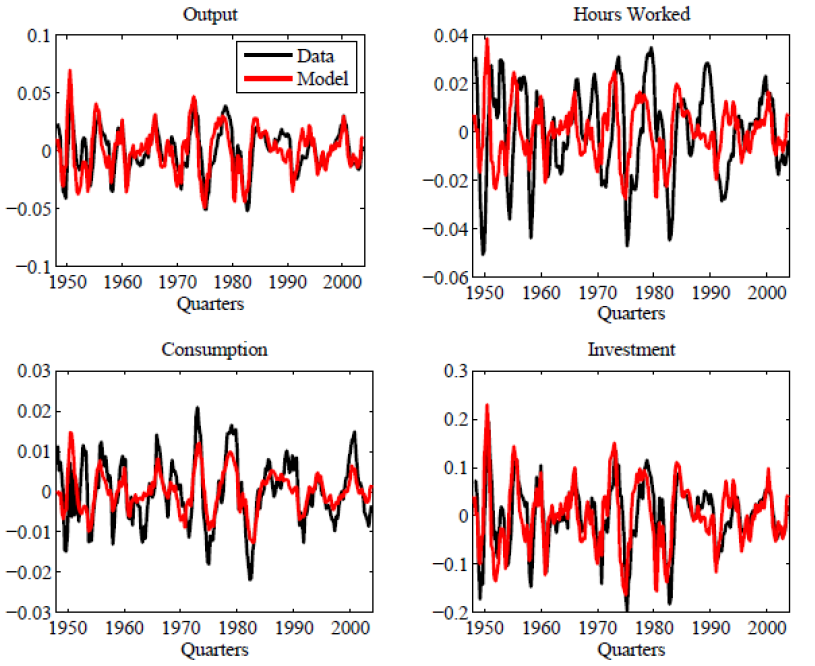
\includegraphics[trim=0 0 0 0,clip,width=0.7\textwidth]{FIGURES/10_RBCestim}
%	}      
%	%\subfigure{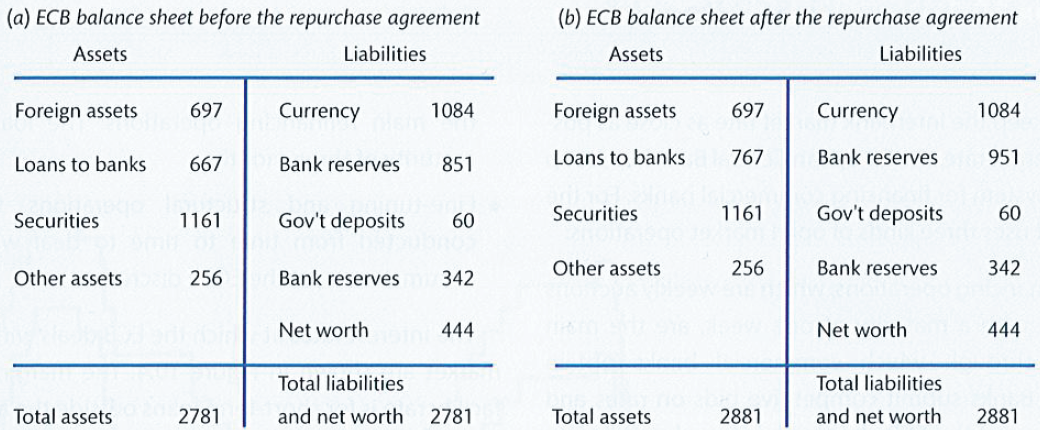
\includegraphics[trim=0 00 0 00,clip,width=0.6\textwidth]{FIGURES/5_CB_balance_sheet_OMO}
%	%} 	
%	%[trim=left bottom right top
%\end{figure}
%%\vspace{-2mm}
%%\begin{minipage}{0.5\columnwidth}
%%\tiny	
%%\textbf{Source.} Burda and Wyplosz (2017), Figure 14.1.\\
%%\end{minipage}
%\end{center}
%
%\end{frame}
%%---FRAME------------------------------------------------------------------------------
%\begin{frame}{Quantitative assessment}
%
%Criticism: Limited internal propagation of a transitory technology shock.
%\begin{center}
%%{\small
%%Figure. 
%%}
%\vspace{-5mm}
%\begin{figure}[h!]
%	\subfigure{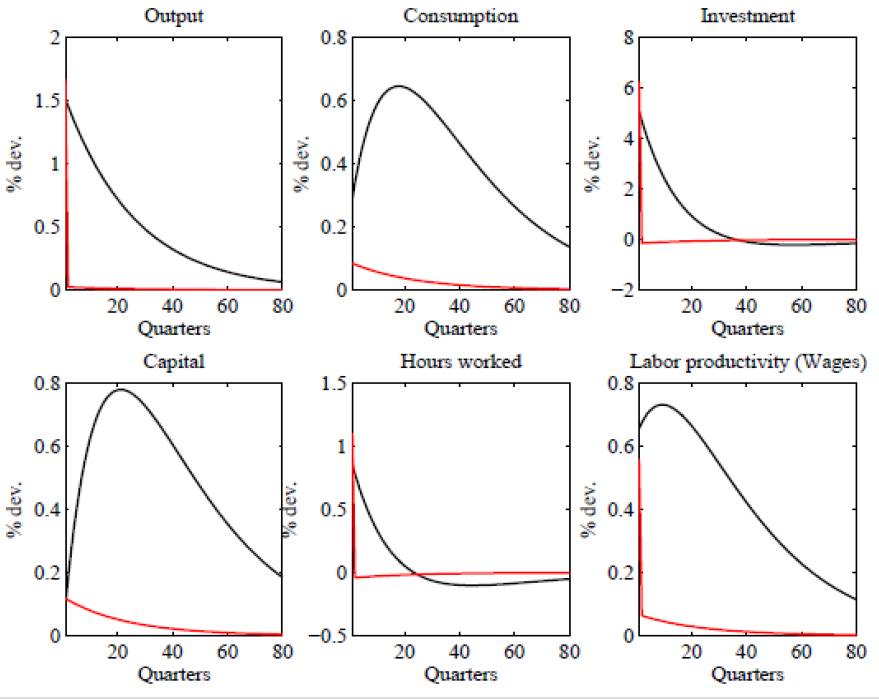
\includegraphics[trim=0 0 0 0,clip,width=0.7\textwidth]{FIGURES/10_RBCpropagation}
%	}      
%	%\subfigure{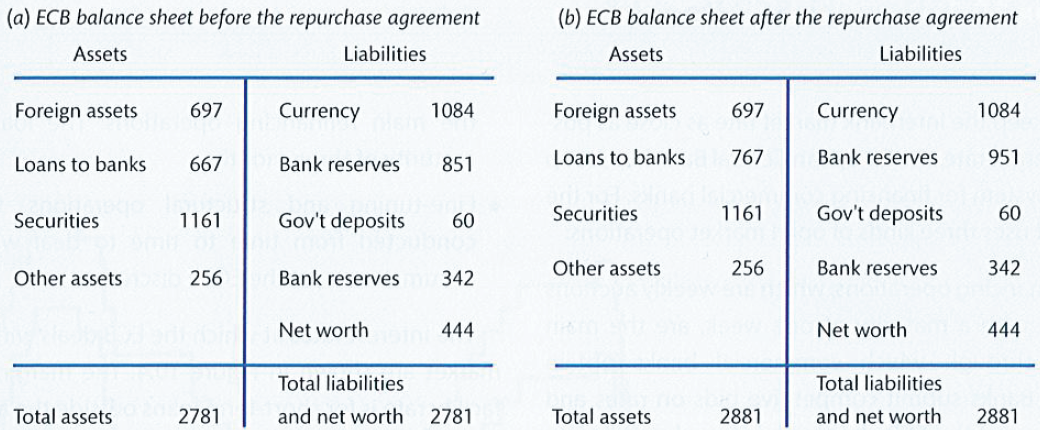
\includegraphics[trim=0 00 0 00,clip,width=0.6\textwidth]{FIGURES/5_CB_balance_sheet_OMO}
%	%} 	
%	%[trim=left bottom right top
%\end{figure}
%%\vspace{-2mm}
%%\begin{minipage}{0.5\columnwidth}
%%\tiny	
%%\textbf{Source.} Burda and Wyplosz (2017), Figure 14.1.\\
%%\end{minipage}
%\end{center}
%
%\end{frame}
%%---FRAME------------------------------------------------------------------------------
%\begin{frame}{Quantitative assessment}
%
%Permanent versus transitory shock
%\begin{center}
%%{\small
%%Figure. 
%%}
%\vspace{-5mm}
%\begin{figure}[h!]
%	\subfigure{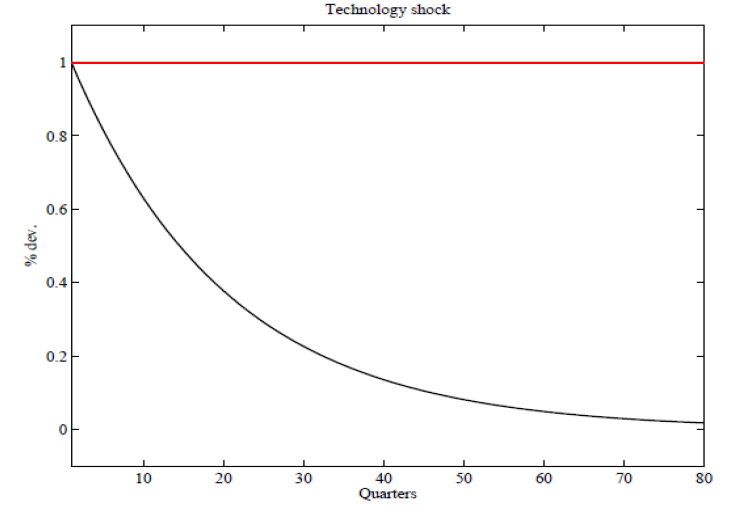
\includegraphics[trim=0 0 0 0,clip,width=0.7\textwidth]{FIGURES/10_IRFshock}
%	}      
%	%\subfigure{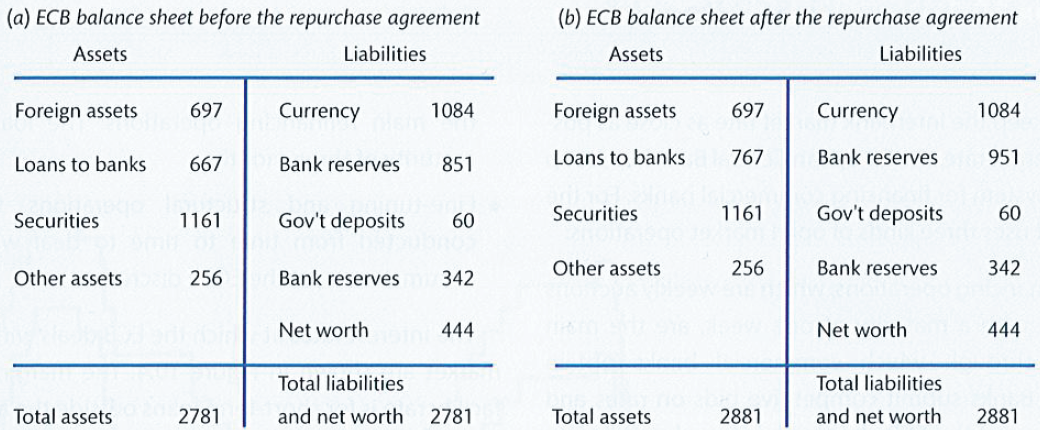
\includegraphics[trim=0 00 0 00,clip,width=0.6\textwidth]{FIGURES/5_CB_balance_sheet_OMO}
%	%} 	
%	%[trim=left bottom right top
%\end{figure}
%%\vspace{-2mm}
%%\begin{minipage}{0.5\columnwidth}
%%\tiny	
%%\textbf{Source.} Burda and Wyplosz (2017), Figure 14.1.\\
%%\end{minipage}
%\end{center}
%
%\end{frame}
%%---FRAME------------------------------------------------------------------------------
%\begin{frame}{Quantitative assessment}
%
%Permanent versus transitory shock: Impulse Response Functions
%\begin{center}
%%{\small
%%Figure. 
%%}
%\vspace{-5mm}
%\begin{figure}[h!]
%	\subfigure{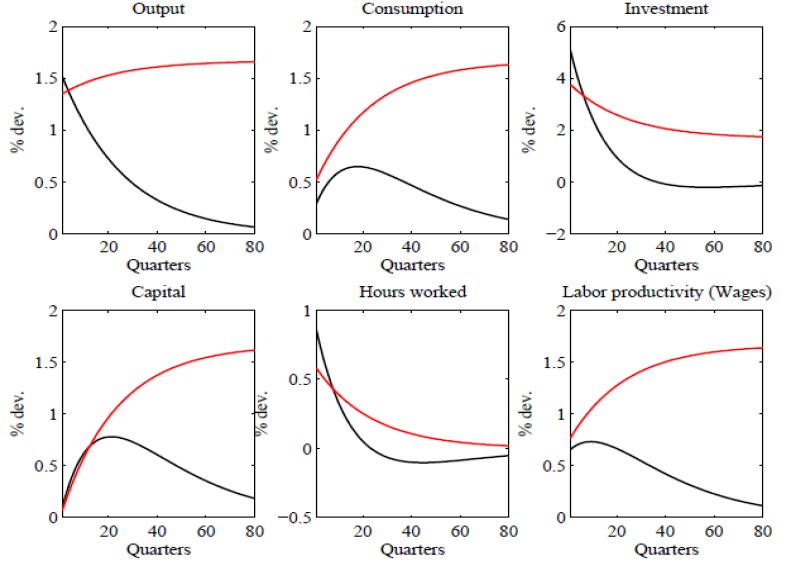
\includegraphics[trim=0 0 0 0,clip,width=0.7\textwidth]{FIGURES/10_IRFresponses}
%	}      
%	%\subfigure{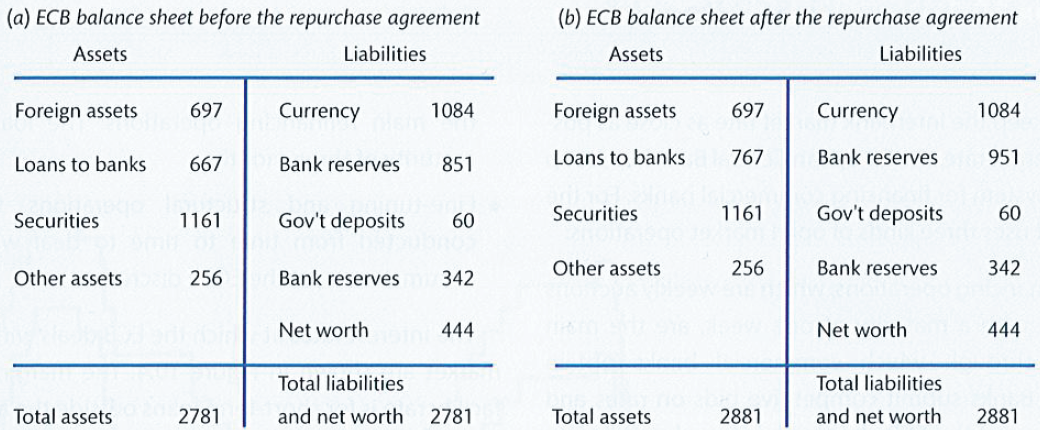
\includegraphics[trim=0 00 0 00,clip,width=0.6\textwidth]{FIGURES/5_CB_balance_sheet_OMO}
%	%} 	
%	%[trim=left bottom right top
%\end{figure}
%%\vspace{-2mm}
%%\begin{minipage}{0.5\columnwidth}
%%\tiny	
%%\textbf{Source.} Burda and Wyplosz (2017), Figure 14.1.\\
%%\end{minipage}
%\end{center}
%
%\end{frame}
%%---FRAME------------------------------------------------------------------------------
%%---END------------------------------------------------------------------------------
\end{document}
